% ****************************************************************************************** % Dissertation template and document class for Princeton University
% Original Author  : Jeffrey Scott Dwoskin <jdwoskin@princeton.edu>
% Adapted from: http://www.math.princeton.edu/graduate/tex/puthesis.html
%
% Adapted for Qatar University by Ryan Riley <ryan.riley@qu.edu.qa>
% ****************************************************************************************** %


\documentclass[12pt,lot,lof]{quthesis}

%%%%%%%%%%%%%%%%%%%%%%%%%%%%%%%%%%%%%%%%%%%%%%%%%%%%%%%%%%%%%\
%%%% Author, title page, and Committee info

\title{Sample Dissertation for Qatar University}

\submitted{June 2013}  % degree conferral date (January or June)
\copyrightyear{2013}  % year in which the copyright is secured by publication of the dissertation.
\author{First Middle Last} % your name
\department{Computer Science and Engineering}
\college{College of Engineering}
\degreetype{Thesis} % Thesis for a master's, Dissertation for a PhD
\degree{Master of Science} % Check with your graduate coordinator for the title of your program's degree.
\adviser{John Smith}  % replace with the full name of your adviser
\committeeone{Bob Jones} % name of first committee member
\committeetwo{Mohamed Ahmed} % name of second committee member


%%%%%%%%%%%%%%%%%%%%%%%%%%%%%%%%%%%%%%%%%%%%%%%%%%%%%%%%%%%%%\
%%%% Tweak float placements
% From: http://mintaka.sdsu.edu/GF/bibliog/latex/floats.html "Controlling LaTeX Floats"
% and based on: http://www.tex.ac.uk/cgi-bin/texfaq2html?label=floats
% LaTeX defaults listed at: http://people.cs.uu.nl/piet/floats/node1.html

% Alter some LaTeX defaults for better treatment of figures:
    % See p.105 of "TeX Unbound" for suggested values.
    % See pp. 199-200 of Lamport's "LaTeX" book for details.
    %   General parameters, for ALL pages:
    \renewcommand{\topfraction}{0.85}	% max fraction of floats at top
    \renewcommand{\bottomfraction}{0.6}	% max fraction of floats at bottom
    %   Parameters for TEXT pages (not float pages):
    \setcounter{topnumber}{2}
    \setcounter{bottomnumber}{2}
    \setcounter{totalnumber}{4}     % 2 may work better
    \setcounter{dbltopnumber}{2}    % for 2-column pages
    \renewcommand{\dbltopfraction}{0.66}	% fit big float above 2-col. text
    \renewcommand{\textfraction}{0.15}	% allow minimal text w. figs
    %   Parameters for FLOAT pages (not text pages):
    \renewcommand{\floatpagefraction}{0.66}	% require fuller float pages
	% N.B.: floatpagefraction MUST be less than topfraction !!
    \renewcommand{\dblfloatpagefraction}{0.66}	% require fuller float pages

% The documentclass already sets parameters to make a high penalty for widows and orphans. 

%%%%%%%%%%%%%%%%%%%%%%%%%%%%%%%%%%%%%%%%%%%%%%%%%%%%%%%%%%%%%\
%%%% Use packages

%\usepackage{amsfonts}

%%% For figures
\usepackage{graphicx}
%\usepackage{subfig,rotate}

%%% for comments
\usepackage{verbatim}

%%% For tables
\usepackage{multirow}
% Longtable lets you have tables that span multiple pages.
\usepackage{longtable}

% Booktabs produces far nicer tables than the standard LaTeX tables.
%   see: http://en.wikibooks.org/wiki/LaTeX/Tables
\usepackage{booktabs}

%set parameters for longtable:
% default caption width is 4in for longtable, but wider for normal tables
\setlength{\LTcapwidth}{\textwidth}

% url package understands urls (with proper line-breaks) without hyperlinking them
\usepackage{url}

%%%%%%%%%%%%%%%%%%%%%%%%%%%%%%%%%%%%%%%%%%%%%%%%%%%%%%%%%%%%%\
%%%% Front-matter

\abstract{
Put your abstract here.
}

\acknowledgements{
Here are all the people you would like to thank.
}

\dedication{
Here are people to dedicate to.
}


%%%%%%%%%%%%%%%%%%%%%%%%%%%%%%%%%%%%%%%%%%%%%%%%%%%%%%%%%%%%%
%%%% Notes:

% Footnotes should be placed after punctuation.\footnote{place here.}
% Generally, place citations before the period~\cite{anotherauthor}.
% The proper usage for i.e., and e.g., include commas ``(e.g., option A, option B)''

%%%%%%%%%%%%%%%%%%%%%%%%%%%%%%%%%%%%%%%%%%%%%%%%%%%%%%%%%%%%%
%%%% Let's build the real document

\begin{document}

\makefrontmatter

\chapter{Introduction}
This document gives you an example of how to produce your Qatar 
University thesis in Latex.  Be sure to read the 
Graduate Academic Manual~\cite{qugam} and make sure that your
final output meets its requirements.

You are not required to follow the sections titles included here by default.
Check the manual (mentioned above) for details.

\begin{table}[t]
\centering
\caption{This is a table caption.  It must be above the table.}
\begin{tabular}{|c|c|}
\hline
Item 1 & Item 2 \\
\hline
Item 3 & Item 4 \\
\hline
\end{tabular}
\end{table}

\begin{figure}[t]
\centering
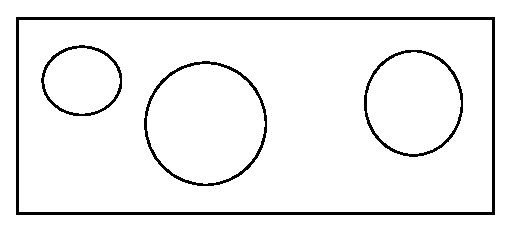
\includegraphics[width=3in]{samplefig.eps}
\caption{This is a figure caption.  It must be below the figure.}
\end{figure}


\chapter{Background and/or Literature Survey}
Your content goes here.

\chapter{Approach/Methodology}
Your content goes here.

\chapter{Implementation/Research Findings}
Your content goes here.

\chapter{Evaluation/Validation}
Your content goes here.

\chapter{Discussion}
Your content goes here.

\chapter{Conclusion}
Your content goes here.

% Make the bibliography single spaced
\singlespacing
\bibliographystyle{plain}

% add the Bibliography to the Table of Contents
\cleardoublepage
\ifdefined\phantomsection
  \phantomsection  % makes hyperref recognize this section properly for pdf link
\else
\fi
\addcontentsline{toc}{chapter}{Bibliography}

% include your .bib file
\bibliography{thesis}

% Appendices if you need them. 

%\appendix
%\chapter{First Appendix}
%Your content goes here.
%\chapter{Second Appendix}
%Your content goes here.

\end{document}

